\documentclass[paper=9in:6in,pagesize=pdftex,headinclude=on,footinclude=on,10pt,bibtotoc,pointlessnumbers,normalheadings,DIV=9,twoside=false]{scrbook}

\areaset[0.50in]{4.5in}{8in}
\KOMAoptions{DIV=last}

\usepackage{trajan}
 
\usepackage[utf8x]{inputenc}
\usepackage[T1]{fontenc}
\usepackage{upgreek}
\usepackage{float}
\usepackage[normal,font={footnotesize,it}]{caption}
\usepackage{graphicx}
\usepackage[sc]{mathpazo}
\linespread{1.05} 
\usepackage[english]{babel}
\usepackage{amsthm}
\usepackage{amsmath}
\usepackage{MnSymbol}
\usepackage{wasysym}
\usepackage{amsfonts}
\newtheorem{theorem}{Theorem}
\renewcommand\qedsymbol{$\blacksquare$}


\begin{document}
\date{}

\begin{center}
\begin{large}
 \textbf{Introduction to the Perceptron\\}
\end{large}
\end{center}
\begin{text} 
Consider a set of vectors $\boldsymbol{\zeta_{\mu}} \in \mathbb{R}^n$, each associated with a
label $\sigma_{\mu}$ .
This is the given information . The $\sigma_{\mu}$ labels takes values ± 1. The simplest perceptron is defined
by a vector of weights \textbf{J} and a  
step functions: $sign(x)$ is the sign of x. The perceptron classifies a vector in a class:
\end{text}
\begin{center}
    $\sigma=sign( \textbf{J} \cdot \boldsymbol{\zeta_{\mu}})$ \\
\end{center}

\begin{text}
The supervision learning problem consists to find the vector of weights \textbf{J} that correctly classifies the vectors $\boldsymbol{\zeta_{\mu}}$ . The vector \textbf{J} is perpendicular to a hyper plane that divide the 2 different labels of vectors.\\
\ \\
\indent The Rosenblatt learning dynamic is given by:
\end{text}

\begin{center}
    $\mathbf{J}(t+1) = \mathbf{J}(t) + \frac{f_\mu}{\sqrt{N}} \cdot  \boldsymbol{\zeta_{\mu}}\sigma_{\mu}$
\end{center}

\begin{text}
where $f_\mu$ is 0 if we have a hit and 1 otherwise. This is an error correction algorithm. \\
\indent If we have a miss, then we update the vector \textbf{J}, if we have a hit, then nothing is done. \\
\indent We shall prove in the next section that if exists a vector \textbf{B} that correctly classifies the vectors $\boldsymbol{\zeta_{\mu}}$ then in a finite number of steps, \textbf{J} converges to \textbf{B}. \\
\ \\
\ \\
\end{text}

\begin{figure}[htb!]
    \centering
    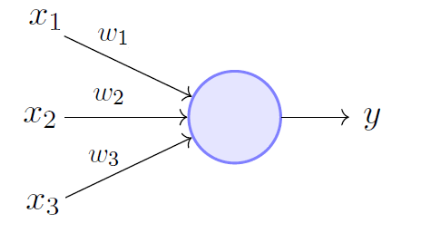
\includegraphics[width=0.4\textwidth]{Screenshot_25.png}
\end{figure}






\end{document}
